\documentclass{scrartcl}

\usepackage[utf8]{inputenc}
\usepackage[T1]{fontenc}
\usepackage{lmodern}
\usepackage[english]{babel}
\usepackage{amsmath}
\usepackage{amssymb}

\usepackage{caption}
\usepackage{graphicx}
\graphicspath{ {./img/} }


\title{Procedural City Generation}
\author{Jakob Krause and Karl Volkenandt}
\begin{document}

\maketitle
\tableofcontents
\newpage


\section{City Generation}
Creating fictional worlds for video games or even urban planning is a task that
can be very expensive and time consuming when done by hand and is hard to change
afterwards on a larger scale.
Procedural city generation attempts to solve this problem by letting algorithms
create the necessary environment. The challenges for generating a city may vary
by application but almost allways has the city to be believable
meaning for example that the structure of the street network should not seem
artificial but rather organic and like something humans could have built.
This often can be achieved by including some degree of randomness in the algorithm.
For tasks like urban planning it does not only have to be believable but also
realistic. The levels of detail can also vary a lot as for some purposes a
city plan may be enough but for others one might want to have different types of
buildings or districts.

When generating a city via procedural methods most of the time we want to have
some degree of freedom concerning the flexibility and parameters we can specify.
For example the size of the city or the density of the buildings and therefore the
population may be parameters that can be used to adjust the city to our liking.
The city may also be generated on a terrain and should look accordingly as it
may be desired that a city evolves around a lake or a sea. This may also vary
since a city may normally avoid mountains but may also favor mountains if it is
supposed to be a small city for mountain farmers.

Also dependent on the application the generation should not be computationally
expensive as it might be important for some games to generate them in real time.




\section{Overview over possible solutions}
There are multiple aproaches to this problem. We prototyped two different solutions.

\subsection{Probability distribution}
One thought was to pick a center for the city and distribute streets and buildings
around it according to a normal distribution so that there is a higher density of streets
and buildings in the middle than further away from the center. This is a rather vague
idea since it does not explain how we would go about creating the street network.

\subsection{Lindenmayer system}
Lindenmayer systems or short L-systems are a way of generating complicated patterns
with only a few given rules that were initially inspired by the way plants evolve.
The basic idea is to give a set of possible symbols that are treated as either variables
or constants and a set of transformation rules describing how variables can be replaced.
Constants are not allowed to be replaced. We then give an initial string (also
called an axiom) and iterate: each symbol of our initial state gets replaced via the given rules.
When done we get a new string consisting of elements of our variables and constants
and repeat the process. After iterating for some time we can stop and need to
translate the output string into an image for example by interpreting every character
of the string as an instruction. Via this method many self similar
structures can be created such as the dragon curve or the Sierpinski triangle.
While this method can give some nice looking and complicated patterns we thought
it would look too artificial when applied to street patterns and did not look further
into it.


\subsection{Agent based}
Another method to generate a believable city that takes care of the street network
and the buildings simultaneously is to simulate the process of
city-generation. This is done in the agent based approach where different agents
move around and interact with the environment based on the local perspective.
Possible agents include street builders, house builders and people investing in certain
areas resulting in industrial quarters or housing areas. This would also add new
buildings but can make the process more complex.



\section{Our approaches}
Before we started thinking how we built our city we wanted to create a terrain
on which the city should be built. We then followed with two approaches to the
city generation and found a way to visualize the results.
From now on everything happens on a two dimensional grid which we wish to fill
with a natural looking city and the terrain around it.

\subsection{Terrain generation using simplex noise}
We decided to use three different tile types for the terrain: Water, grass and mountain.
For terrain generation we used a simplex noise. This is a noise that is similar
to the computationally more expensive Perlin noise which is used for tasks like
procedural texture generation and is used in the terrain generation of the computer
game Minecraft. This noise is procedurally generated the result is not random. To
obtain mentioned randomness and get different terrains we generate
a three dimensional simplex noise and use only a random two dimensional slice as our terrain.
Using this method we get some natural looking two dimensional terrains.
\begin{figure}
  \centering
  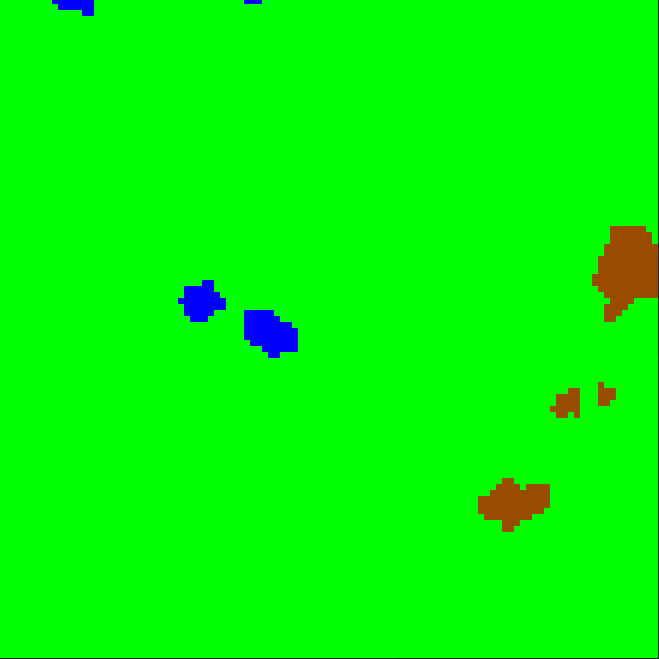
\includegraphics[scale = 0.2]{terrain_example}
  \caption{An example of a terrain generated by simplex noise \\Blue = Water, Green = Grass, Brown = Mountain}
\end{figure}
The next step is to figure out where we can start to build the city. This is done
by assigning a grade to each point on the grid and starting the city at the point
with the highest score. This is done by specifying a radius (vaguely giving
the size of the city) and checking for each point how much area of grass,
water and mountain is contained in a circle of the given radius.
We decided that starting a city near mountain is not preferred and thus the number
of tiles representing mountains is subtracted from the score. Conversely the area
of grass is added to the score. For water we thought that a certain amount of water
is preferred over too much or too little water. To realize this we add a weighted score based
on the difference of the preferred amount of water and the real amount of water in
the circle. The preferred amount of water is given by a percentage that should be
covered in water. This percentage then influences how far away from water the
city will be built.
\begin{figure}
  \centering
  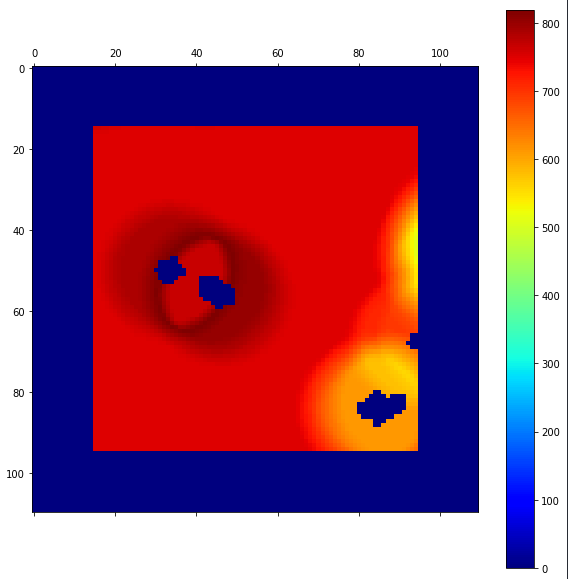
\includegraphics[scale = 0.25]{heatmap_citycenter}
  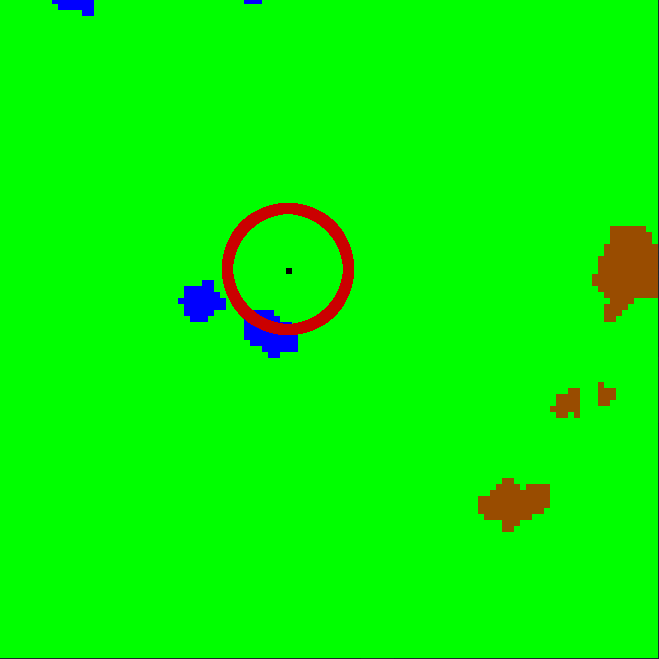
\includegraphics[scale = 0.2]{terrain_citycenter_circle}
  \caption{(left) A heatmap visualizing the score assigned to each position on the map\\
          (right) the final chosen point inside the red circle where the city will be built}
\end{figure}

\subsection{Agent based}
To pursue the idea of an agent based system we would first like to have a street
leading to the center of the city. This makes thematically sense since cities do not get
built in the middle of nothing. To do this we select a random point on the border
of our map and connect it with a street to the city center. To achieve this in a way
that does not look artificial we equally distribute points every few tiles on
the straight line between the point on the border and the point chosen to be our
city center. We then move these points by a small random amount and use them as the
control points if a bezier curve forming the street coming from the outside to
the city.

We now introduce two types of agents to our map: The street builder and the house builder.
All agents have a method telling them where to move and a method telling them
how to change the environment. The way how they determine where to move is very similar.
Theoretically the agents look at each direction they can move (one tile north, east, south or west)
and assign a score to them. We then look at the two largest scores and the agent
moves towards one of the two directions at random with a higher chance of choosing
the direction in which the maximum score is assigned. This is done in order to
get rid of the deterministic movement and allow for multiple agents to move along
different paths. Instead of just looking at the relevant positions on the map we
look at each and every single point on our map and evaluate a score. That way we
can plot this scoremap and estimate how the agents will move based on the given
parameters.

Both agents rate the positions based on the number of different tile types in a
circle of given radius. The street builders get a street density as parameter
that influences the score the same way water influences the heatmap explained before.
This rule alone results in streets that run parallel to each other. In order to
get streets between these parallel streets we let the number of built houses nearby
positively influence the score. If we are given the scenario just described
a house builder will most likely build some buildings between the two streets.
Now the street builders are incentivised to build a street close to the buildings
connecting the parallel streets.
We want to have streets that have enough free space for buildings around them
so grass increases the score. Finally to give the city some tendency to a shape
we let the distance of the street builder to the origin of the city influence the score.
After a street builder moves he builds a street at his current location.

The house builders are only allowed to move on streets but we allow them to build
in a small radius around them allowing for more than one row of buildings along a street.
The score the house builders use is positively influenced by water, streets, the
distance to the city origin and grass. This is because it is attractive to live
near the water or midtown where the density of streets should be a bit higher.
The number of buildings in the neighborhood reduces the score resulting in movement
away from developed part to places with space to build. After moving a house gets built
at a random position in a small circle around the agent.

All that is left to do now is to let a given amount of street builders spawn at the
city center and let them start  building the street network. We gave the agents
a lifetime to prevent them from filling up the whole map. The house builders
have a much shorter lifetime than the street builders but after dying at each location
of the street builders a house builder spawns resulting in residential neighborhoods.

\begin{figure}
  \centering
  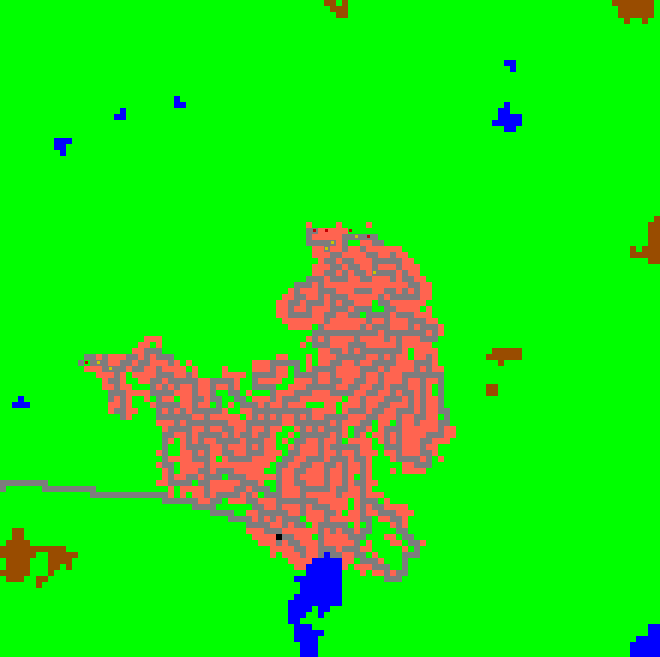
\includegraphics[scale = 0.2]{city}
  \caption{A city generated by an agent based system}
\end{figure}

The sheer amount of parameters of approach allows for a lot of fine tuning.
It is however not easy to give meta parameters such as city size or an amount
of area that should be covered by buildings. However the results look very organic
and due to the random nature not artificial. We made use of two different tile types
inside the city, namely streets and buildings. This could potentially be extended
by different types of buildings such as skyscrapers that get built in higher
populated areas. The simulation could also be extended by adding monetary variables
and using them to influence were different kind of buildings get built.

\subsection{Procedural street networks by Voronoi diagramms}

Another valid option for creating a street network is to use Voronoi diagrams.
In our case the diagram is a partion of the 2-dimensional euclidian plane.
Every element of the partion is a voronoi cell.
A voronoi cell of a  $ P \subset \mathbb{R}^2 $ and a distance function $d$ is defined as

\[
    V_k=\lbrace \forall x \in \mathbb{R}^2 \mid d(x,p_k) \leq d(x,p_i)), \forall i \ne k \land p_i,p_k \in P ) \rbrace
\]

\begin{figure}
    \centering
    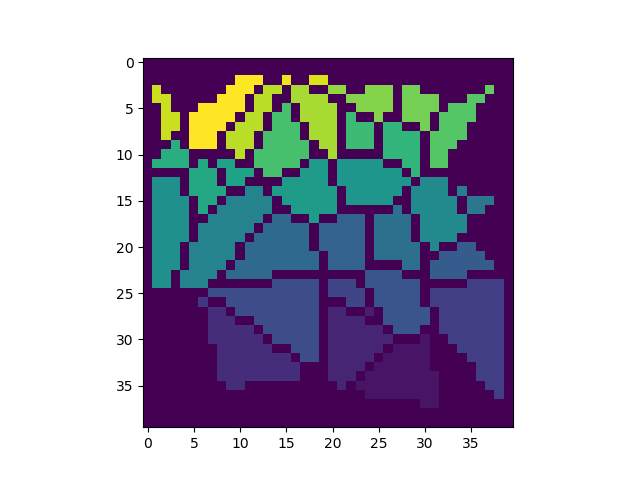
\includegraphics[scale = 0.5]{voro}
    \caption{A sampled street network generated by a voronoi diagram
    the different colors show the single voronoi cells $V_k$}
    \label{fig:voronoi}
\end{figure}

A voronoi digram is a the set of $V_k$ over $P$.
Our general idea now is to create a voronoi diagram for some random points
and to use the edges as streets in our city. Further we wan to fill up the
space inside the cell with buildings.

We  start with a set of random point $P$ (uniform distribution) of a given
size $n$. The next step would be to create the voronoi diagram $V$ of $P$.
The datastructure of the diagram is now the set of edges of our cells.
The span of this diagram is usally much bigger than our furthest points from $P$.
So we need to specify which part of the $V$ we want to use for further processing.
The most interresting part of the diagram happens in the smallest bounding
box of $P$. A bounding box is a rectangle which
accomodates all points in $P$. We cut out all edge with ending points outside
of the bounding box.

Since our city is build of an $n\times n$ grid we need to raster our edges.
We used the classic Bresenham line algorithm to draw lines between the edge points.
An example can be seen in figure~\ref{fig:voronoi}.

Since having just some streets filled with standart houses looks a little
generic we added some random pole points to our city.
A pole points mean that in the area around the point there is a higher change
for having a skyscrapper instead of a standart house. The chance is represented
by a 2D-normal distribution.
The amount of pole points can be set as a parameter in our generator.

\begin{figure}
    \centering
    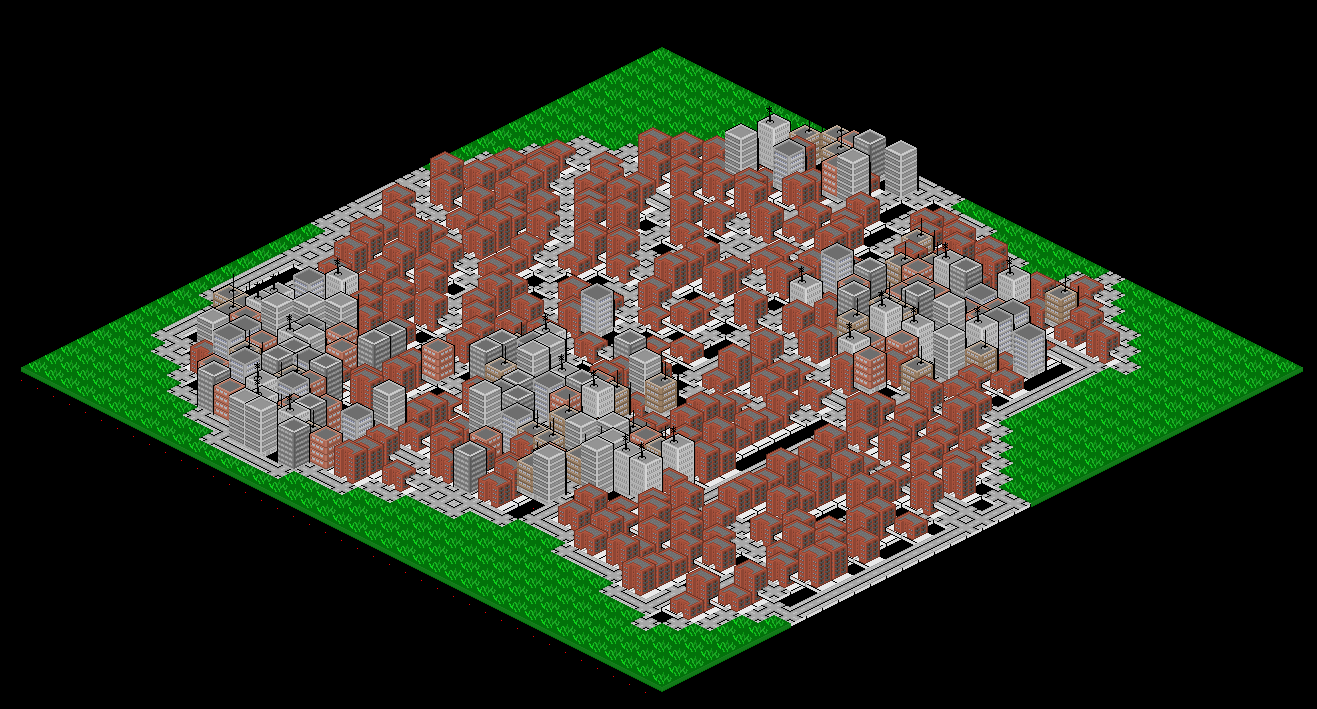
\includegraphics[scale = 1.2]{city1}
    \caption{Possible outcome of our city generator. Here we have choosen 4 pole
    points so we received 4 regions with skyscrappers.}
    \label{fig:city_example}
\end{figure}

The final results can be seen in figure~\ref{fig:city_example}.


\subsection{Plotting}
Tileplotting mittels pygame, anfangs nur Farbkästen, dann sprites werden auch
wenn es mal wieder Zeit ist




\end{document}
